%
% $RCSfile: theory.tex,v $
%
% Copyright (c) 2002-2007. Christian Heller. All rights reserved.
%
% Permission is granted to copy, distribute and/or modify this document
% under the terms of the GNU Free Documentation License, Version 1.1 or
% any later version published by the Free Software Foundation; with no
% Invariant Sections, with no Front-Cover Texts and with no Back-Cover
% Texts. A copy of the license is included in the section entitled
% "GNU Free Documentation License".
%
% http://www.cybop.net
% - Cybernetics Oriented Programming -
%
% Version: $Revision: 1.1 $ $Date: 2007-08-01 13:59:01 $ $Author: christian $
% Authors: Christian Heller <christian.heller@tuxtax.de>
%

\section{Theory}
\label{theory_heading}
\index{CYBOP}
\index{Theory}

The theory behind CYBOL is called \emph{Cybernetics Oriented Programming}
(CYBOP). It describes the general concepts, software architecture and
development principles that justify the existence of CYBOL. Besides CYBOL as
language, CYBOP suggests the \emph{Cybernetics Oriented Interpreter} (CYBOI).

\begin{figure}[ht]
    \begin{center}
        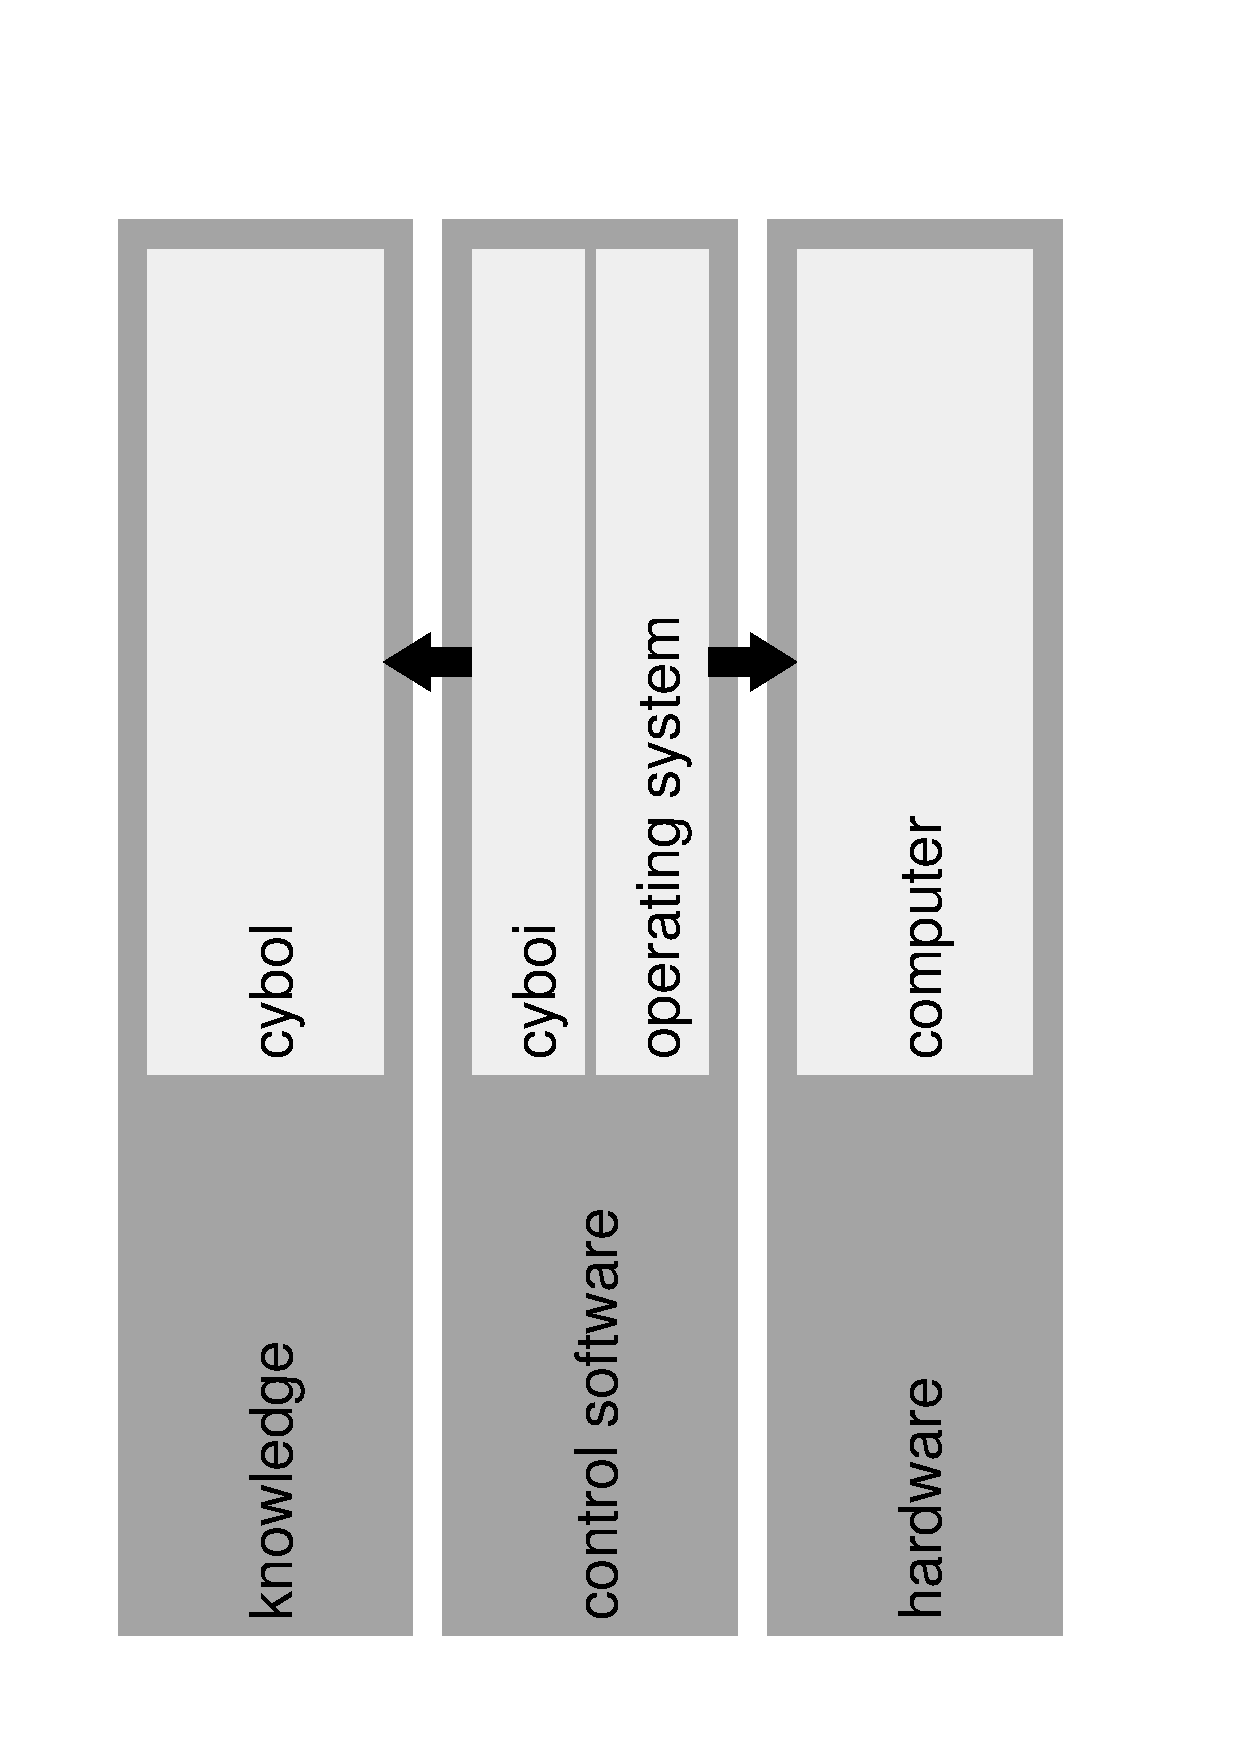
\includegraphics[scale=0.3,angle=-90]{graphics/interpretation.pdf}
        \caption{CYBOL Interpretation}
        \label{interpretation_figure}
    \end{center}
\end{figure}

Considering an overall computer system architecture, \emph{CYBOI} as low-level
software system is situated between the application knowledge existing in form
of \emph{CYBOL} templates and the \emph{Hardware} controlled by an
\emph{Operating System} (OS), as is shown in figure \ref{interpretation_figure}.
CYBOI as \emph{active} system process interprets the \emph{passive} application
knowledge provided in form of CYBOL files.

Design-time knowledge resides in CYBOL \emph{Knowledge Templates} (files).
While being instantiated, it gets transferred into runtime
\emph{Knowledge Models} that reside in a computer's \emph{Random Access Memory}
(RAM).
